\HydraSection[
  focus x=0.62,
  focus y=0.44,
  radius=0.12,
  zoom=1.90
]{Reaction--diffusion approach}

\HydraSubsection[
  Chemical signals provide a natural mechanism for spatial organization.
]{Chemical  \mbox{patterning}}

\begin{frame}{Could chemical signals determine where a head forms?}

  \HydraTextImage[5.65cm]{
    \vspace{0.5cm}
    \HydraPoint[HydraGold]
      {Cells communicate through chemical signals}
      {Signaling molecules can be produced, transformed and removed by cells.}

    \vspace{0.18cm}

    \HydraPoint[HydraCyan]
      {Concentrations can vary in space}
      {Different regions of the tissue may therefore experience different levels of the same signal.}

    \vspace{0.18cm}

    \HydraPoint[HydraGold]
      {A local maximum can select a site}
      {A sufficiently high concentration may trigger head-forming activity in one particular region.}

    \vspace{0.18cm}

    \HydraPoint[HydraCyan]
      {Chemistry can position the organizer}
      {{The location of head formation becomes a question of how a spatial concentration pattern arises.}}

  }
  {figures/B_reaction_diffusion/Concentration.png}
  {}

  \vspace{0.10cm}

  % \HydraTakeaway{
  %   One possible mechanism is that a spatial pattern of chemical signals
  %   selects the position of the head organizer.
  % }

\end{frame}


\begin{frame}{Reactions change signals, diffusion moves them}

  \vspace{0.30cm}

  \begin{columns}[T,onlytextwidth]

    \begin{column}{0.46\textwidth}

      {\color{HydraGold}\bfseries
       \fontsize{11.5}{13.5}\selectfont
       REACTION\par}

      \vspace{0.35cm}

      \HydraPoint[HydraGold]
        {Local chemical change}
        {Cells can produce, remove or transform signaling molecules.}

      \vspace{0.25cm}

      \HydraPoint[HydraGold]
        {Local feedback}
        {The production of a signal may depend on the concentrations already present in the same region.}

    \end{column}

    \begin{column}{0.46\textwidth}

      {\color{HydraCyan}\bfseries
       \fontsize{11.5}{13.5}\selectfont
       DIFFUSION\par}

      \vspace{0.35cm}

      \HydraPoint[HydraCyan]
        {Spatial redistribution}
        {Signaling molecules spread from regions of higher concentration toward regions of lower concentration.}

      \vspace{0.25cm}

      \HydraPoint[HydraCyan]
        {Communication across tissue}
        {Diffusion couples nearby regions, allowing a local chemical change to influence its surroundings.}

    \end{column}

  \end{columns}

  \vfill

  % \HydraTakeaway{
  %   Pattern formation becomes possible when local chemical feedback
  %   is coupled to spatial communication.
  % }

\end{frame}




\begin{frame}{Mechanism of chemical pattern formation}

  \vspace{0.12cm}

  \begin{columns}[c,onlytextwidth]

    % ----------------------------------------------------------
    % Turing + original paper
    % ----------------------------------------------------------
    \begin{column}{0.29\textwidth}
      \centering

      \begin{minipage}{0.72\linewidth}
        \centering
        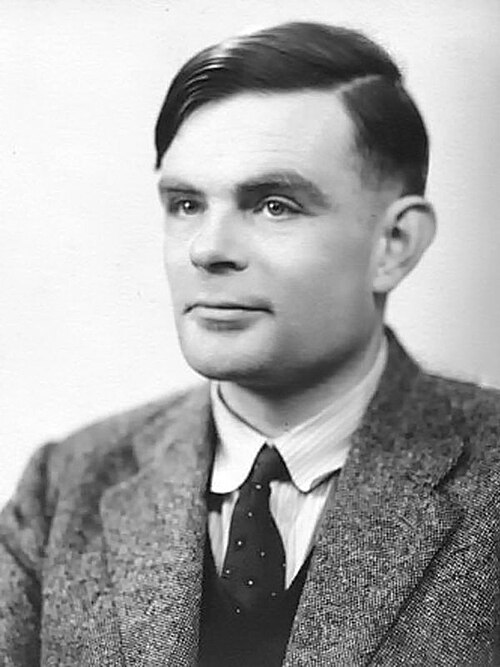
\includegraphics[
          width=\linewidth,
          height=2.35cm,
          keepaspectratio
        ]{figures/common/Alan_Turing_(1951).jpg}
      \end{minipage}

      \vspace{0.08cm}

      {\color{HydraGold}\bfseries
       \fontsize{19}{22}\selectfont 1952\par}

      {\color{HydraWhite}\bfseries
       \fontsize{9.5}{11}\selectfont Alan Turing\par}

      \vspace{0.18cm}

      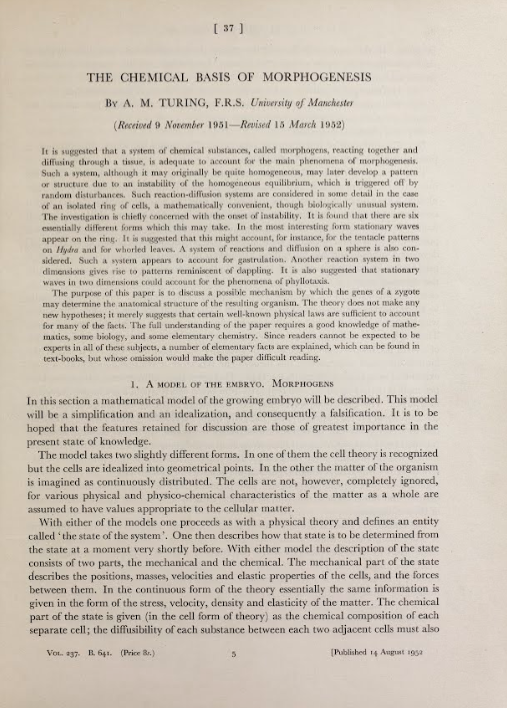
\includegraphics[
        width=0.66\linewidth,
        height=2.15cm,
        keepaspectratio
      ]{figures/B_reaction_diffusion/TuringPaper.png}

    \end{column}

    % ----------------------------------------------------------
    % Main message
    % ----------------------------------------------------------
    \begin{column}{0.65\textwidth}

      \HydraPoint[HydraGold]
        {A homogeneous tissue need not stay homogeneous}
        {Chemical substances can react and diffuse through tissue, allowing spatial structure to emerge from small perturbations.}

      \vspace{0.18cm}

      \HydraPoint[HydraCyan]
        {Diffusion becomes part of the mechanism}
        {Spatial transport is not merely smoothing: together with reactions it can participate in pattern formation.}

      \vspace{0.18cm}

      \HydraPoint
        {Hydra was already on the list}
        {Turing explicitly mentioned stationary patterns as a possible explanation for tentacle organization in Hydra.}

    \end{column}

  \end{columns}

  \vspace{0.15cm}

  \HydraTakeaway{
    Reaction and diffusion can, in principle, turn an almost homogeneous state into spatial structure
  }
  
  % \vspace{0.40cm}
  % \source{
    % A.~M. Turing, \textit{Phil. Trans. R. Soc. B} 237 (1952), 37--72.
    % Portrait: Elliott \& Fry, 1951, Wikimedia Commons.
  % }

\end{frame}

\begin{frame}{Gierer and Meinhardt propose a model}

  \vspace{0.15cm}

  \begin{columns}[T,onlytextwidth]

    % ----------------------------------------------------------
    % Portraits
    % ----------------------------------------------------------
    \begin{column}{0.30\textwidth}
      \centering

      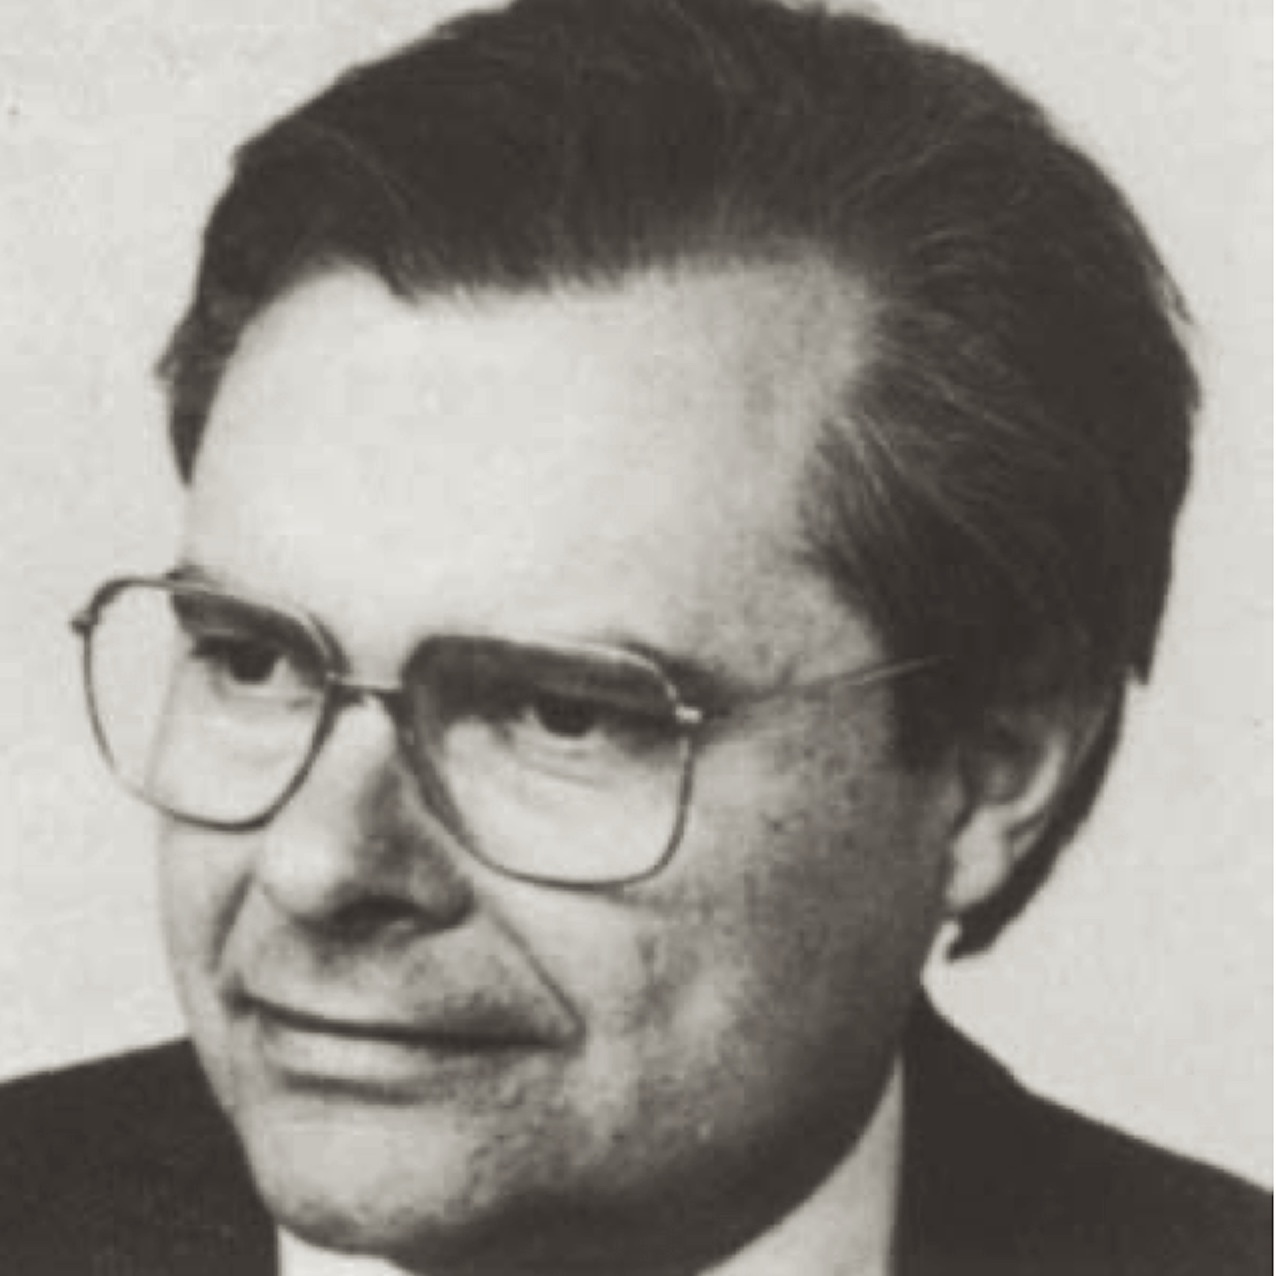
\includegraphics[
        width=0.72\linewidth,
        height=2.25cm,
        keepaspectratio
      ]{figures/B_reaction_diffusion/Alfred_Gierer.jpg}

      \vspace{0.07cm}

      {\color{HydraWhite}\bfseries\fontsize{8.5}{10}\selectfont
        Alfred Gierer\par}

      \vspace{0.28cm}

      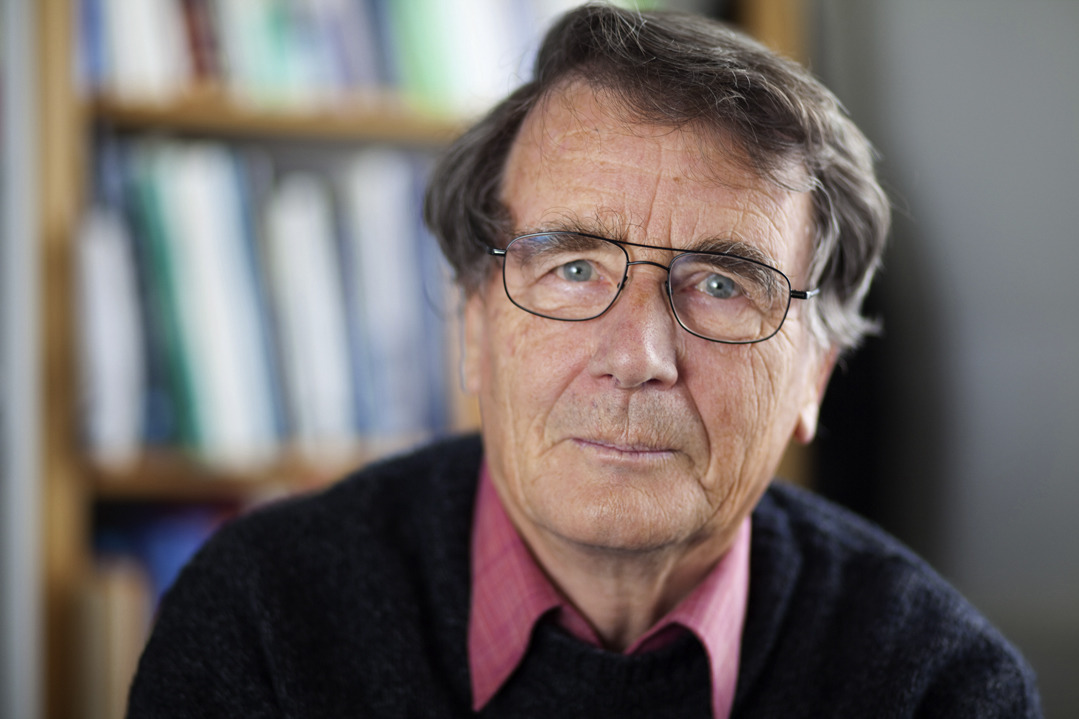
\includegraphics[
        width=0.72\linewidth,
        height=2.25cm,
        keepaspectratio
      ]{figures/B_reaction_diffusion/Hans_Meinhardt.jpg}

      \vspace{0.07cm}

      {\color{HydraWhite}\bfseries\fontsize{8.5}{10}\selectfont
        Hans Meinhardt\par}

    \end{column}

    % ----------------------------------------------------------
    % Paper + mechanism
    % ----------------------------------------------------------
    \begin{column}{0.64\textwidth}

      {\color{HydraGold}\bfseries\fontsize{9}{10.5}\selectfont
        A. GIERER \& H. MEINHARDT   /   1972 \par}

      \vspace{0.08cm}

      {\color{HydraWhite}\bfseries\fontsize{15}{18}\selectfont
        \textit{A Theory of Biological Pattern Formation}\par}

      \vspace{0.18cm}

      {\color{HydraMuted}\fontsize{8.2}{10.5}\selectfont
        A mechanism for generating spatial organization
        in an initially almost homogeneous tissue.\par}

      \vspace{0.48cm}

      \HydraPoint[HydraGold]
        {Local self-activation}
        {A small local excess reinforces itself and can develop into a localized organizing region.}

      \vspace{0.30cm}

      \HydraPoint[HydraCyan]
        {Long-range inhibition}
        {The activated region generates an inhibitory effect that acts over a larger spatial range.}

    \end{column}

  \end{columns}

  \source{
    Gierer \& Meinhardt,
    \textit{Kybernetik} 12 (1972), 30--39.
  }

\end{frame}

\begin{frame}{The activator--inhibitor idea}

  \begin{center}
    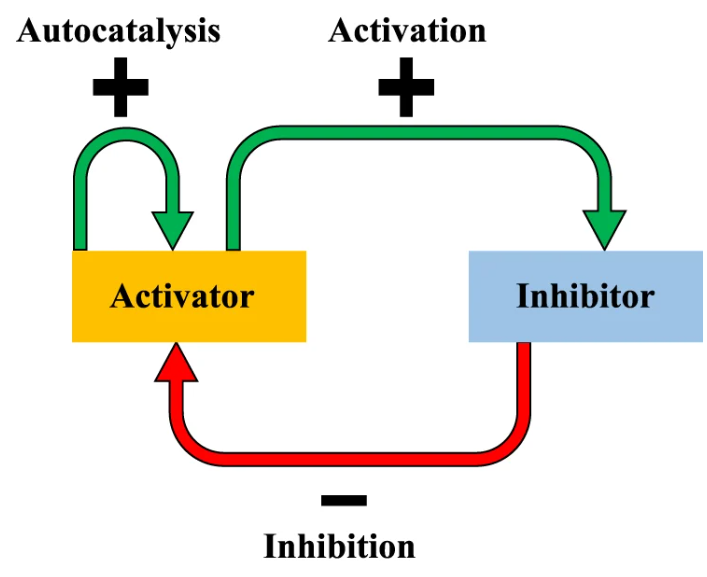
\includegraphics[
      width=0.85\textwidth,
      height=5.5cm,
      keepaspectratio
    ]{figures/B_reaction_diffusion/ActivatorInhibitor.png}

    % \vspace{0.05cm}

    % {\color{HydraMuted}\fontsize{6}{7.2}\selectfont
      % Schematic illustration of local activation and long-range inhibition.\par}
  \end{center}

  \vspace{0.08cm}

  \begin{columns}[T,onlytextwidth]

    \begin{column}{0.47\textwidth}
      \HydraPoint[HydraGold]
        {Activator}
        {Enhances its own production and promotes local organizer formation. Its effect remains relatively localized.}
    \end{column}

    \begin{column}{0.47\textwidth}
      \HydraPoint[HydraCyan]
        {Inhibitor}
        {Is produced by activated regions, suppresses further activation and acts over a longer spatial range.}
    \end{column}

  \end{columns}

\end{frame}



\begin{frame}{The Gierer--Meinhardt model}

  \vspace{-0.50cm}

  \begin{columns}[c,onlytextwidth]

    % ----------------------------------------------------------
    % Equations
    % ----------------------------------------------------------
    \begin{column}{0.65\textwidth}

      {\color{HydraWhite}\fontsize{12.5}{17}\selectfont
      \begin{align*}
        \partial_t u
        &=
        \underbrace{
          D_u\Delta u
        }_{\color{HydraCyan}\text{diffusion}}
        \quad+\quad
        \underbrace{
          \frac{a u^2}{K+v}-\mu_u u
        }_{\color{HydraGold}\text{reaction}}
        \\[0.75cm]
        \partial_t v
        &=
        \underbrace{
          D_v\Delta v
        }_{\color{HydraCyan}\text{diffusion}}
        \quad+\quad
        \underbrace{
          b u^2-\mu_v v
        }_{\color{HydraGold}\text{reaction}}
      \end{align*}
      }

    \end{column}

    % ----------------------------------------------------------
    % Variables
    % ----------------------------------------------------------
    \begin{column}{0.30\textwidth}
      \vspace{0.10cm}

      \HydraPoint[HydraGold]
        {$u$: activator}
        {Promotes its own production and initiates local organizer activity}

      \vspace{0.55cm}

      \HydraPoint[HydraCyan]
        {$v$: inhibitor}
        {Produced by the activator and suppresses its production}

    \end{column}

  \end{columns}

  \vspace{0.25cm}

  % ----------------------------------------------------------
  % Parameters
  % ----------------------------------------------------------
  {\color{HydraWhite}\fontsize{8.8}{11.3}\selectfont

  \begin{columns}[t,onlytextwidth]

    \begin{column}{0.47\textwidth}

      \textcolor{HydraCyan}{$D_u,\;D_v$}
      \quad diffusion rates, typically $D_v>D_u$

      \vspace{0.18cm}

      \textcolor{HydraGold}{$a$}
      \quad strength of activator self-amplification

      \vspace{0.18cm}

      \textcolor{HydraGold}{$b$}
      \quad strength of inhibitor production

    \end{column}

    \begin{column}{0.47\textwidth}

      \textcolor{HydraGold}{$K$}
      \quad scale of inhibition by $v$

      \vspace{0.18cm}

      \textcolor{HydraGold}{$\mu_u$}
      \quad activator degradation rate

      \vspace{0.18cm}

      \textcolor{HydraGold}{$\mu_v$}
      \quad inhibitor degradation rate

    \end{column}

  \end{columns}
  }

\end{frame}

\begin{frame}{A general reaction--diffusion system}

  \vspace{0.10cm}

  \begin{columns}[c,onlytextwidth]

    \begin{column}{0.65\textwidth}
      {\color{HydraWhite}\fontsize{12.5}{17}\selectfont
      \begin{align*}
        \partial_t u
        &=
        \underbrace{D_u\Delta u}_{\color{HydraCyan}\text{diffusion}}
        \quad+\quad
        \underbrace{f(u,v)}_{\color{HydraGold}\text{reaction}},
        \\[0.75cm]
        \partial_t v
        &=
        \underbrace{D_v\Delta v}_{\color{HydraCyan}\text{diffusion}}
        \quad+\quad
        \underbrace{g(u,v)}_{\color{HydraGold}\text{reaction}}.
      \end{align*}
      }
    \end{column}

    \begin{column}{0.30\textwidth}
      \HydraPoint[HydraGold]
        {$u$ and $v$}
        {Concentrations of two interacting chemical signals.}

      \vspace{0.38cm}

      \HydraPoint[HydraGold]
        {$f$ and $g$}
        {Possibly nonlinear local production, removal and interaction terms.}
    \end{column}

  \end{columns}

  \vfill

  \HydraTakeaway{
    We begin by deriving the spatial transport term
  }

\end{frame}

\HydraSubsection[
  \mbox{Diffusion redistributes signals} \mbox{through space and smooths} \mbox{concentration differences}
]{Diffusion}





\begin{frame}{Diffusion begins with a local balance}

  \vspace{0.25cm}

  \begin{columns}[c,onlytextwidth]

    \begin{column}{0.32\textwidth}
      \HydraPoint[HydraCyan]
        {Concentration}
        {$u(x,t)$ measures the amount of a substance per unit length at point $x$.}

      \vspace{0.38cm}

      \HydraPoint[HydraGold]
        {Control volume}
        {We track the substance inside a short interval of length $\Delta x$.}
    \end{column}

    \begin{column}{0.64\textwidth}
      \centering
      \begin{tikzpicture}[x=1cm,y=1cm]
        \fill[HydraPanel,rounded corners=5pt]
          (0.15,0.70) rectangle (8.15,3.15);
        \draw[HydraLine,line width=0.8pt,rounded corners=5pt]
          (0.15,0.70) rectangle (8.15,3.15);

        \foreach \x in {0.70,1.45,2.20,2.95,3.70,4.45,5.20,5.95,6.70,7.45}{
          \draw[HydraLine,line width=0.45pt]
            (\x,0.72) -- (\x,3.13);
        }

        \fill[HydraGold,opacity=0.18]
          (3.05,0.72) rectangle (5.18,3.13);
        \draw[HydraGold,line width=1.15pt]
          (3.05,0.62) -- (3.05,3.26);
        \draw[HydraGold,line width=1.15pt]
          (5.18,0.62) -- (5.18,3.26);

        \foreach \px/\py in {0.55/2.55,0.92/1.35,1.28/2.20,1.68/1.75,
          2.05/2.70,2.45/1.20,2.72/2.05,3.35/2.48,
          3.78/1.42,4.22/2.18,4.72/1.75,5.55/2.52,
          6.02/1.32,6.46/2.10,7.04/1.70,7.58/2.42}{
          \fill[HydraCyan] (\px,\py) circle[radius=0.055cm];
        }

        \node[anchor=south,text=HydraWhite,
          font=\bfseries\fontsize{9.5}{11}\selectfont]
          at (4.12,3.38) {$u(x,t)$};
        \node[anchor=north,text=HydraGold,
          font=\bfseries\fontsize{8}{9.5}\selectfont]
          at (3.05,0.48) {$x$};
        \node[anchor=north,text=HydraGold,
          font=\bfseries\fontsize{8}{9.5}\selectfont]
          at (5.18,0.48) {$x+\Delta x$};

        \draw[<->,>=Latex,HydraGold,line width=0.8pt]
          (3.12,0.0) -- (5.11,0.0);
        \node[text=HydraGold,font=\fontsize{8}{9.5}\selectfont]
          at (4.12,-0.18) {$\Delta x$};
      \end{tikzpicture}

      \vspace{0.15cm}

      {\color{HydraWhite}\fontsize{11.5}{14}\selectfont
        \[
          \text{amount in the interval}
          \;\approx\;
          u(x,t)\,\Delta x
        \]
      }
    \end{column}

  \end{columns}

\end{frame}


\begin{frame}{Boundary flux}

  \vspace{0.12cm}

  \begin{columns}[c,onlytextwidth]

    \begin{column}{0.74\textwidth}
      \centering
      \begin{tikzpicture}[x=0.78cm,y=0.82cm]
        \fill[HydraPanel,rounded corners=5pt]
          (2.15,1.18) rectangle (9.15,3.82);
        \draw[HydraLine,line width=0.9pt,rounded corners=5pt]
          (2.15,1.18) rectangle (9.15,3.82);
        \fill[HydraGold,opacity=0.14]
          (2.18,1.21) rectangle (9.12,3.79);

        \draw[HydraGold,line width=1.2pt]
          (2.15,0.98) -- (2.15,4.02);
        \draw[HydraGold,line width=1.2pt]
          (9.15,0.98) -- (9.15,4.02);

        \draw[-{Latex[length=3mm]},HydraCyan,line width=2.0pt]
          (0.38,2.50) -- (2.02,2.50);
        \draw[-{Latex[length=3mm]},HydraCyan,line width=2.0pt]
          (9.28,2.50) -- (10.92,2.50);

        \node[anchor=south,text=HydraCyan,
          font=\bfseries\fontsize{10}{11.5}\selectfont]
          at (1.18,2.78) {$J(x,t)$};
        \node[anchor=south,text=HydraCyan,
          font=\bfseries\fontsize{10}{11.5}\selectfont]
          at (10.52,2.78) {$J(x+\Delta x,t)$};

        \foreach \px/\py in {2.65/3.14,3.08/1.72,3.62/2.52,4.18/3.28,
          4.72/1.68,5.28/2.70,5.82/1.92,6.38/3.16,
          6.95/2.28,7.52/3.24,8.05/1.65,8.62/2.55}{
          \fill[HydraWhite] (\px,\py) circle[radius=0.06cm];
        }

        \node[anchor=north,text=HydraGold,
          font=\bfseries\fontsize{8}{9.5}\selectfont]
          at (2.15,0.82) {$x$};
        \node[anchor=north,text=HydraGold,
          font=\bfseries\fontsize{8}{9.5}\selectfont]
          at (9.15,0.82) {$x+\Delta x$};
      \end{tikzpicture}

      \vspace{0.10cm}

      {\color{HydraMuted}\fontsize{8.4}{10}\selectfont
        \textcolor{HydraCyan}{\bfseries Flux $J$:}
        amount of substance crossing a boundary.
      \par}

      \vspace{0.12cm}

      {\color{HydraWhite}\fontsize{11.2}{14.5}\selectfont
      \[
        \frac{
          u(x,t+\Delta t)\,\Delta x-u(x,t)\,\Delta x
        }{\Delta t}
        =
        \textcolor{HydraCyan}{J(x,t)}
        -
        \textcolor{HydraCyan}{J(x+\Delta x,t)}
      \]
      }
    \end{column}

    \begin{column}{0.22\textwidth}
      {\color{HydraMuted}\fontsize{7.1}{8.7}\selectfont
        \textcolor{HydraWhite}{$J(x,t)>J(x+\Delta x,t)$}
        \par
        \vspace{0.04cm}
        amount increases

        \vspace{0.42cm}

        \textcolor{HydraWhite}{$J(x,t)=J(x+\Delta x,t)$}
        \par
        \vspace{0.04cm}
        amount stays constant

        \vspace{0.42cm}

        \textcolor{HydraWhite}{$J(x,t)<J(x+\Delta x,t)$}
        \par
        \vspace{0.04cm}
        amount decreases
      }
    \end{column}

  \end{columns}

  \vfill

  \HydraTakeaway{
    Only a difference between the boundary fluxes changes the amount inside
  }

\end{frame}


\begin{frame}{The local conservation law}

  \vspace{0.08cm}

  \begin{center}
    \begin{tikzpicture}[x=0.78cm,y=0.82cm]
      \fill[HydraPanel,rounded corners=5pt]
        (2.15,1.18) rectangle (9.15,3.82);
      \draw[HydraLine,line width=0.9pt,rounded corners=5pt]
        (2.15,1.18) rectangle (9.15,3.82);
      \fill[HydraGold,opacity=0.14]
        (2.18,1.21) rectangle (9.12,3.79);

      \draw[HydraGold,line width=1.2pt]
        (2.15,0.98) -- (2.15,4.02);
      \draw[HydraGold,line width=1.2pt]
        (9.15,0.98) -- (9.15,4.02);

      \draw[-{Latex[length=3mm]},HydraCyan,line width=2.0pt]
        (0.38,2.50) -- (2.02,2.50);
      \draw[-{Latex[length=3mm]},HydraCyan,line width=2.0pt]
        (9.28,2.50) -- (10.92,2.50);

      \node[anchor=south,text=HydraCyan,
        font=\bfseries\fontsize{10}{11.5}\selectfont]
        at (1.18,2.78) {$J(x,t)$};
      \node[anchor=south,text=HydraCyan,
        font=\bfseries\fontsize{10}{11.5}\selectfont]
        at (10.52,2.78) {$J(x+\Delta x,t)$};

      \foreach \px/\py in {2.65/3.14,3.08/1.72,3.62/2.52,4.18/3.28,
        4.72/1.68,5.28/2.70,5.82/1.92,6.38/3.16,
        6.95/2.28,7.52/3.24,8.05/1.65,8.62/2.55}{
        \fill[HydraWhite] (\px,\py) circle[radius=0.06cm];
      }

      \node[anchor=north,text=HydraGold,
        font=\bfseries\fontsize{8}{9.5}\selectfont]
        at (2.15,0.82) {$x$};
      \node[anchor=north,text=HydraGold,
        font=\bfseries\fontsize{8}{9.5}\selectfont]
        at (9.15,0.82) {$x+\Delta x$};
    \end{tikzpicture}
  \end{center}

  \vspace{-0.58cm}

  \begin{center}
    {\color{HydraWhite}\fontsize{11.5}{15}\selectfont
    \[
      \frac{u(x,t+\Delta t)-u(x,t)}{\Delta t}
      =
      -\frac{
        \textcolor{HydraCyan}{J(x+\Delta x,t)}
        -\textcolor{HydraCyan}{J(x,t)}
      }{\Delta x}
    \]
    }

    \vspace{-0.10cm}

\begin{center}
  {\color{HydraCyan}\fontsize{18}{18}\selectfont
    $\Downarrow$
    \rlap{%
      \hspace{0.25cm}%
      {\fontsize{9.5}{11.5}\selectfont
        $\Delta t,\Delta x\longrightarrow0$%
      }%
    }
  \par}
\end{center}

    \vspace{-0.72cm}

    {\color{HydraWhite}\bfseries\fontsize{17}{21}\selectfont
    \[
      \boxed{\partial_tu=-\partial_xJ}
    \]
    }
  \end{center}

\end{frame}


\begin{frame}{Fick's law of diffusion}

  \vspace{0.04cm}

  \begin{columns}[c,onlytextwidth]

    \begin{column}{0.27\textwidth}
      \centering

      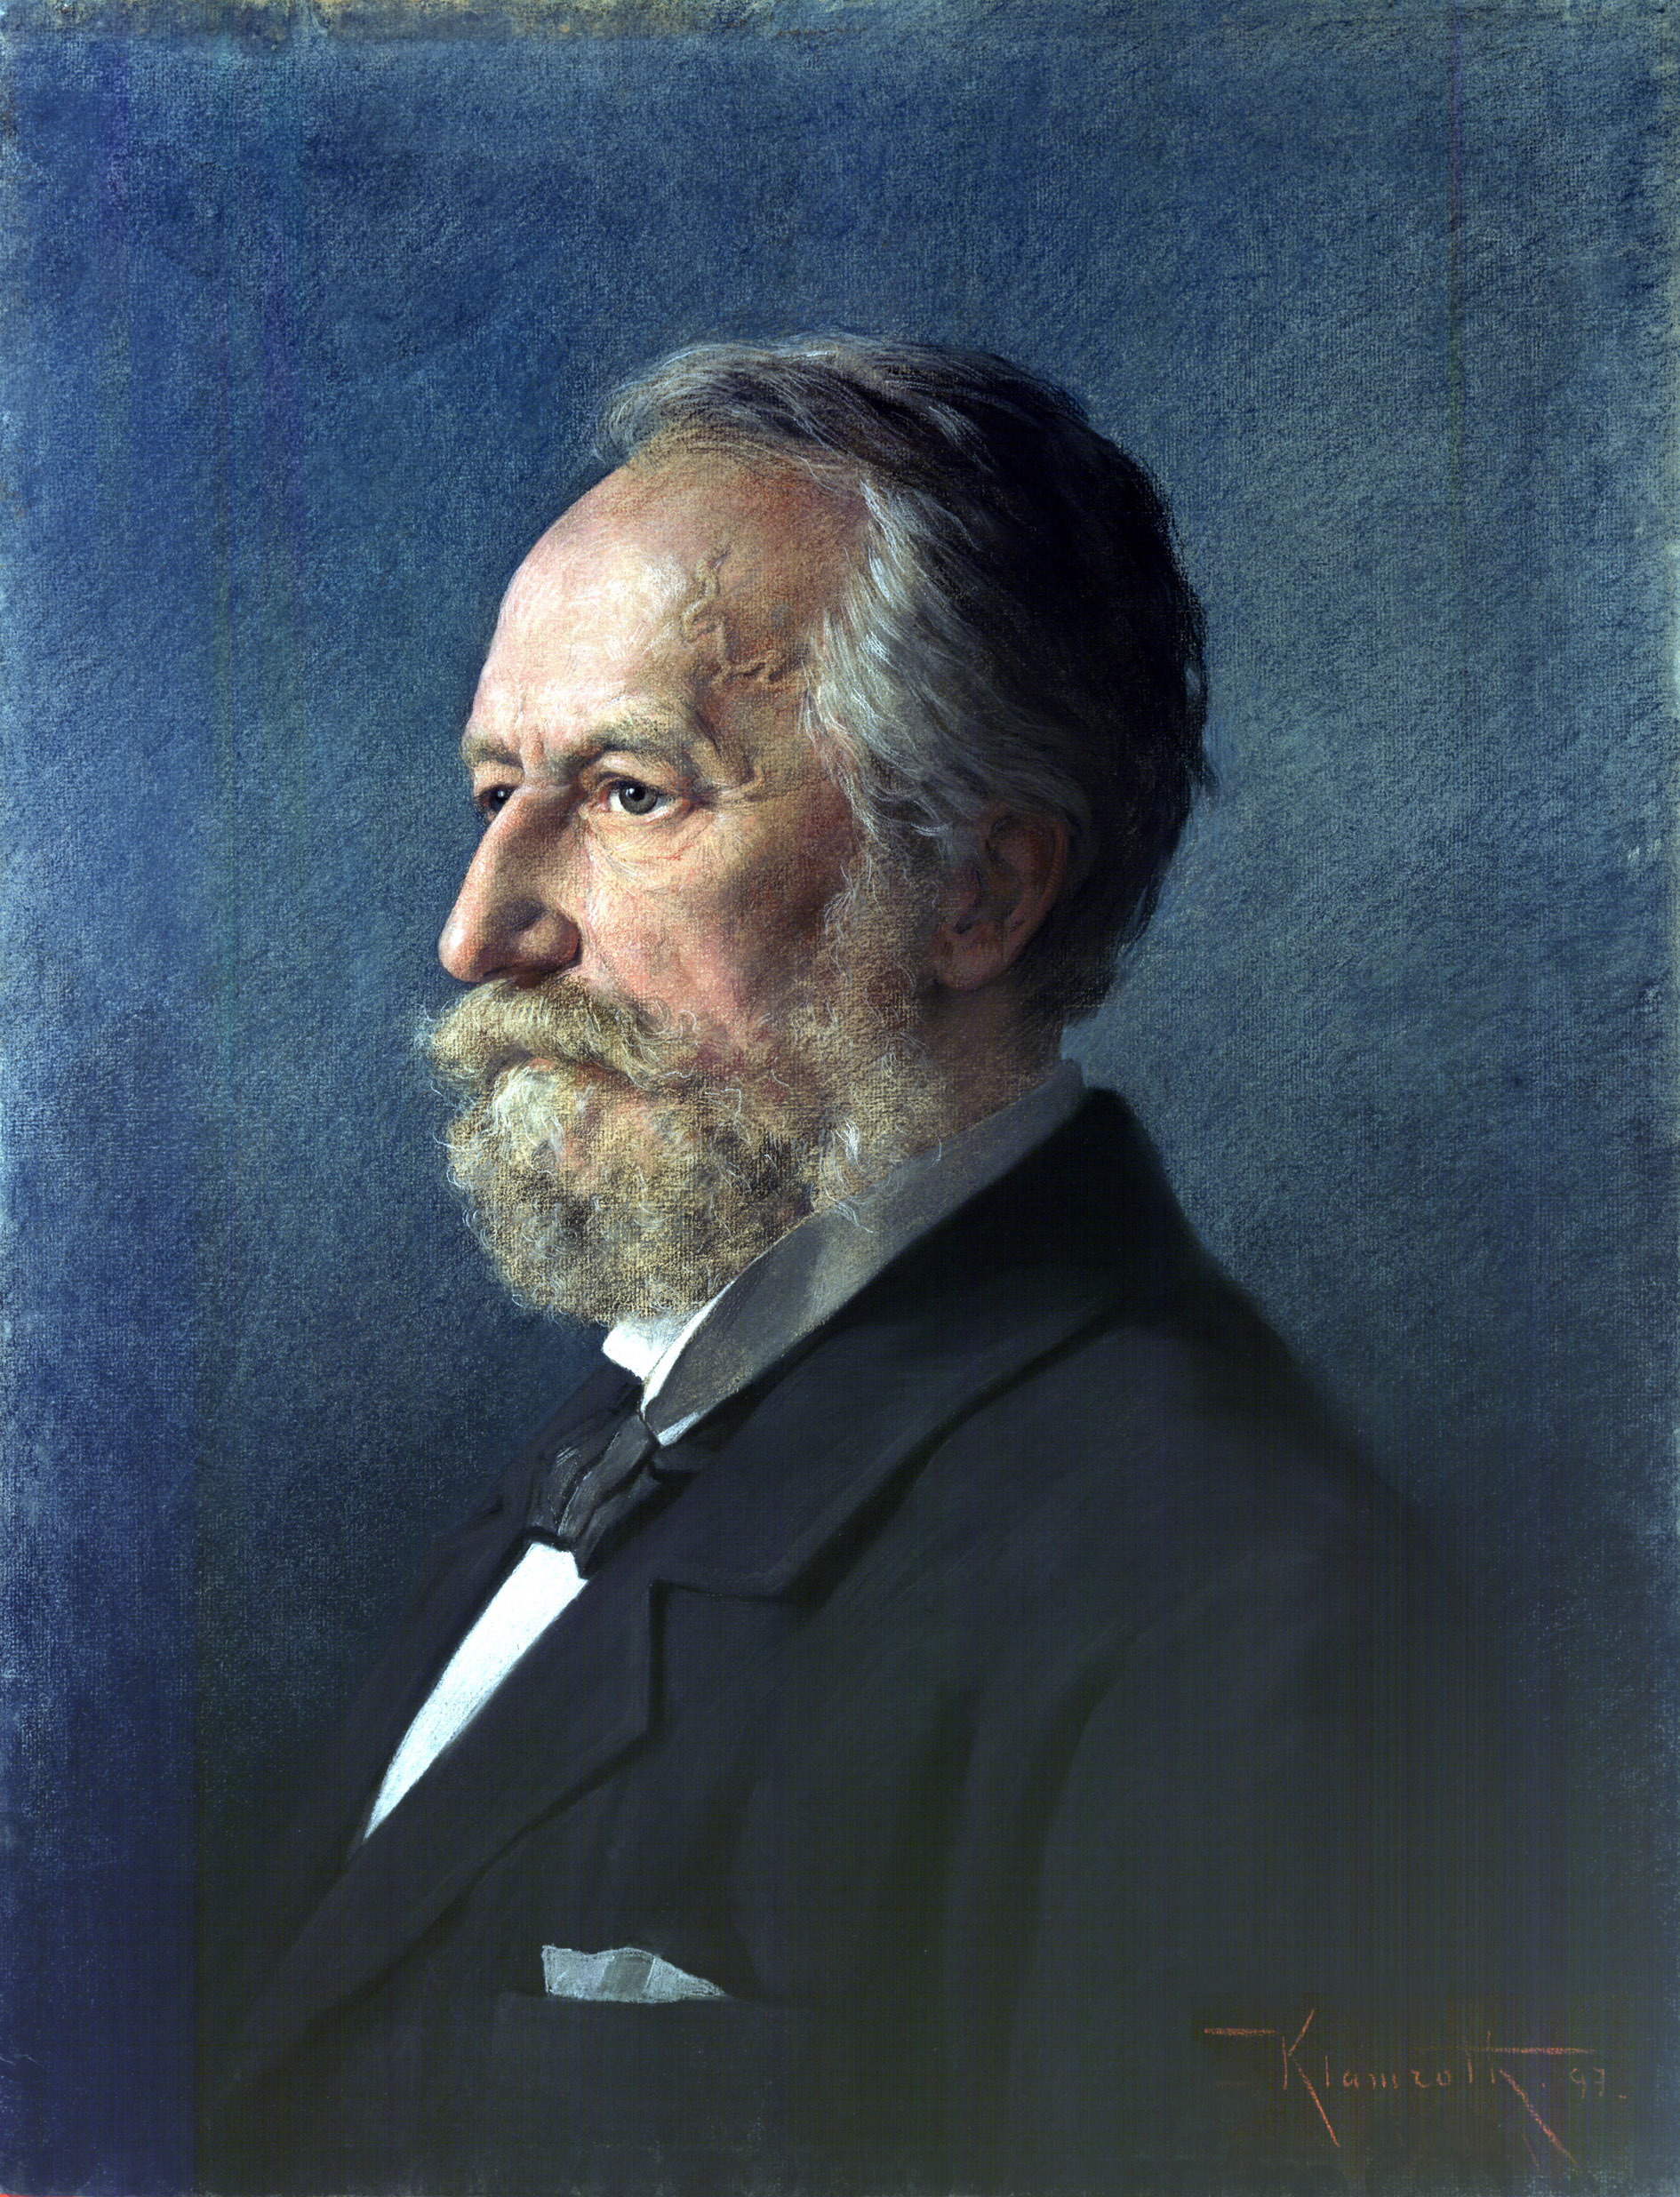
\includegraphics[
        width=0.70\linewidth,
        height=2.65cm,
        keepaspectratio
      ]{figures/B_reaction_diffusion/Adolf_Fick_1897.jpg}

      \vspace{0.05cm}

      {\color{HydraWhite}\bfseries\fontsize{9}{10.5}\selectfont
        ADOLF FICK
      \par}
      {\color{HydraMuted}\fontsize{7.2}{8.5}\selectfont
        1829--1901
      \par}

      \vspace{0.16cm}

      {\color{HydraGold}\bfseries\fontsize{15}{17}\selectfont
        1855
      \par}

      \vspace{0.02cm}

      {\color{HydraWhite}\bfseries\fontsize{10.5}{12.5}\selectfont
        \textit{Ueber Diffusion}
      \par}

      \vspace{0.14cm}

      {\color{HydraMuted}\fontsize{7.6}{9.5}\selectfont
        Using Fourier's heat-conduction analogy,
        Fick related diffusive flux to the
        concentration gradient
      \par}


    \end{column}

    \begin{column}{0.69\textwidth}
            \vspace{-2.18cm}

      \begin{center}
        {\color{HydraWhite}\bfseries\fontsize{15}{18}\selectfont
        \[
          \boxed{J=-D\,\partial_xu}
        \]
        }
      \end{center}

      \vspace{-0.8cm}
      \centering
      \begin{tikzpicture}[x=0.95cm,y=0.88cm]
        \draw[-{Latex[length=2.4mm]},HydraMuted,line width=0.8pt]
          (0.45,0.55) -- (7.25,0.55)
          node[below,text=HydraMuted,font=\fontsize{8}{9}\selectfont] {$x$};
        \draw[-{Latex[length=2.4mm]},HydraMuted,line width=0.8pt]
          (0.55,0.45) -- (0.55,4.80)
          node[left,text=HydraMuted,font=\fontsize{8}{9}\selectfont] {$u(x)$};

        \draw[HydraGold,line width=1.8pt]
          plot[smooth] coordinates {
            (0.65,4.30) (1.25,4.08) (1.95,3.78) (2.65,3.38)
            (3.35,2.92) (4.05,2.42) (4.75,1.92) (5.45,1.48)
            (6.15,1.12) (6.85,0.88)
          };

        \draw[HydraWhite,dashed,line width=0.8pt]
          (2.55,3.58) -- (5.18,1.67);
        \fill[HydraWhite] (3.85,2.64) circle[radius=0.06cm];
        \node[anchor=south west,text=HydraWhite,
          font=\fontsize{8}{9.5}\selectfont]
          at (3.92,2.72) {negative gradient};

        \node[anchor=south west,text=HydraGold,
          font=\bfseries\fontsize{7.5}{9}\selectfont]
          at (0.82,4.28) {HIGH};
        \node[anchor=south east,text=HydraGold,
          font=\bfseries\fontsize{7.5}{9}\selectfont]
          at (6.32,0.60) {LOW};

        \draw[-{Latex[length=3mm]},HydraCyan,line width=2.2pt]
          (2.30,0.05) -- (5.25,0.05);
        \node[anchor=north,text=HydraCyan,
          font=\bfseries\fontsize{9}{10.5}\selectfont]
          at (3.78,-0.12) {flux $J$};
      \end{tikzpicture}

      \vspace{-0.0cm}

      \begin{columns}[T,totalwidth=\linewidth]
        \begin{column}{0.32\linewidth}
          \centering
          {\color{HydraWhite}\fontsize{8.1}{9.7}\selectfont
            $\partial_xu<0\Rightarrow J>0$
          \par}
          {\color{HydraMuted}\fontsize{6.8}{8.2}\selectfont
            flux to the right
          \par}
        \end{column}

        \begin{column}{0.32\linewidth}
          \centering
          {\color{HydraWhite}\fontsize{8.1}{9.7}\selectfont
            $\partial_xu=0\Rightarrow J=0$
          \par}
          {\color{HydraMuted}\fontsize{6.8}{8.2}\selectfont
            no concentration-driven flux
          \par}
        \end{column}

        \begin{column}{0.32\linewidth}
          \centering
          {\color{HydraWhite}\fontsize{8.1}{9.7}\selectfont
            $|J|=D\,|\partial_xu|$
          \par}
          {\color{HydraMuted}\fontsize{6.8}{8.2}\selectfont
            steeper gradient, larger flux
          \par}
        \end{column}
      \end{columns}

    \end{column}

  \end{columns}

  % \source{
  %   A. Fick, \textit{Ueber Diffusion}, \textit{Annalen der Physik} 170 (1855), 59--86.
  %   Portrait: Anton Klamroth, 1897, Wikimedia Commons (public domain).
  % }

\end{frame}


\begin{frame}{Diffusion equation}

  \vspace{0.02cm}

  \begin{columns}[c,onlytextwidth]
    \begin{column}{0.36\textwidth}
      \centering
      {\color{HydraGold}\bfseries\fontsize{7.6}{9}\selectfont
        LOCAL CONSERVATION\par}
      \vspace{0.04cm}
      {\color{HydraWhite}\fontsize{11.5}{14}\selectfont
        $\partial_tu=-\partial_xJ$
      \par}
    \end{column}

    \begin{column}{0.05\textwidth}
      \centering
      {\color{HydraCyan}\fontsize{15}{15}\selectfont $+$}
    \end{column}

    \begin{column}{0.36\textwidth}
      \centering
      {\color{HydraGold}\bfseries\fontsize{7.6}{9}\selectfont
        FICK'S LAW\par}
      \vspace{0.04cm}
      {\color{HydraWhite}\fontsize{11.5}{14}\selectfont
        $J=-D\partial_xu$
      \par}
    \end{column}
  \end{columns}

  \vspace{0.06cm}

  \begin{center}
    {\color{HydraCyan}\fontsize{16}{16}\selectfont $\Downarrow$\par}

    \vspace{0.66cm}

    {\color{HydraGold}\bfseries\fontsize{8.4}{10}\selectfont
      DIFFUSION EQUATION\par}

    \vspace{0.12cm}

    {\color{HydraWhite}\bfseries\fontsize{20}{24}\selectfont
      $\boxed{\partial_tu=D\partial_{xx}u}$
    \par}
  \end{center}

\end{frame}


\begin{frame}{The diffusion equation on a bounded domain}

  \vspace{0.04cm}

  \begin{columns}[c,onlytextwidth]

    \begin{column}{0.40\textwidth}
      % {\color{HydraGold}\bfseries\fontsize{8}{9.5}\selectfont
        % ONE-DIMENSIONAL PROBLEM\par}

      % \vspace{0.10cm}

      % {\color{HydraMuted}\fontsize{8.2}{10}\selectfont
      %   $x\in(0,L),\qquad t>0$
      % \par}

      % \begin{center}
        {\color{HydraMuted}\fontsize{9}{11}\selectfont
          $\Omega=[0,L]\subset\mathbb{R}$
        \par}
      % \end{center}

      \vspace{-0.52cm}

      {\color{HydraWhite}\fontsize{12.5}{16.5}\selectfont
      \begin{align*}
        \partial_tu(x,t) &= D\,\partial_{xx}u(x,t),
        \\[0.24cm]
        u(x,0) &= u_0(x).
      \end{align*}
      }
    \end{column}

    \begin{column}{0.64\textwidth}
      \centering
      \begin{tikzpicture}[x=0.88cm,y=0.60cm]
        \draw[-{Latex[length=2.2mm]},HydraMuted,line width=0.7pt]
          (0.35,0.45) -- (7.70,0.45)
          node[below,text=HydraMuted,font=\fontsize{7}{8.2}\selectfont] {$x$};
        \draw[-{Latex[length=2.2mm]},HydraMuted,line width=0.7pt]
          (0.45,0.35) -- (0.45,3.70)
          node[left,text=HydraMuted,font=\fontsize{7}{8.2}\selectfont] {$u(x,t)$};

        \draw[HydraGold,line width=1.7pt]
          plot[smooth] coordinates {
            (0.60,0.52) (1.50,0.54) (2.30,0.64) (2.95,1.05)
            (3.42,2.10) (3.75,3.42) (4.08,2.10) (4.55,1.05)
            (5.20,0.64) (6.00,0.54) (7.45,0.52)
          };
        \draw[HydraWhite,line width=1.35pt]
          plot[smooth] coordinates {
            (0.60,0.56) (1.42,0.64) (2.20,0.88) (2.88,1.38)
            (3.42,2.04) (3.75,2.38) (4.08,2.04) (4.62,1.38)
            (5.30,0.88) (6.08,0.64) (7.45,0.56)
          };
        \draw[HydraCyan,line width=1.55pt]
          plot[smooth] coordinates {
            (0.60,0.64) (1.35,0.82) (2.08,1.08) (2.78,1.40)
            (3.35,1.67) (3.75,1.75) (4.15,1.67) (4.72,1.40)
            (5.42,1.08) (6.15,0.82) (7.45,0.64)
          };

        \node[anchor=west,text=HydraGold,
          font=\bfseries\fontsize{7}{8.2}\selectfont]
          at (4.10,3.28) {$t=0$};
        \node[anchor=west,text=HydraWhite,
          font=\bfseries\fontsize{7}{8.2}\selectfont]
          at (4.48,2.18) {$t=t_1$};
        \node[anchor=west,text=HydraCyan,
          font=\bfseries\fontsize{7}{8.2}\selectfont]
          at (5.15,1.52) {$t=t_2$};
      \end{tikzpicture}
    \end{column}

  \end{columns}

  \vspace{0.98cm}

  \begin{columns}[T,onlytextwidth]

    \begin{column}{0.47\textwidth}
      \HydraPoint[HydraCyan]
        {No-flux boundary (Neumann)}
        {The sealed ends prevent the substance from leaving}

      \vspace{0.05cm}

      \centering
      \begin{tikzpicture}[x=0.85cm,y=0.70cm]
        \fill[HydraPanel,rounded corners=3pt]
          (0.55,0.55) rectangle (7.00,1.65);
        \draw[HydraLine,line width=0.75pt,rounded corners=3pt]
          (0.55,0.55) rectangle (7.00,1.65);

        \draw[HydraGold,line width=2.0pt]
          (0.55,0.45) -- (0.55,1.75);
        \draw[HydraGold,line width=2.0pt]
          (7.00,0.45) -- (7.00,1.75);

        \foreach \px/\py in {0.95/1.28,1.45/0.82,2.02/1.38,2.58/0.92,
          3.18/1.25,3.72/0.76,4.28/1.38,4.88/0.96,5.45/1.30,6.08/0.80,6.58/1.28}{
          \fill[HydraCyan] (\px,\py) circle[radius=0.055cm];
        }

        \node[anchor=north,text=HydraMuted,
          font=\fontsize{6.8}{8}\selectfont] at (0.55,0.38) {$x=0$};
        \node[anchor=north,text=HydraMuted,
          font=\fontsize{6.8}{8}\selectfont] at (7.00,0.38) {$x=L$};
      \end{tikzpicture}
      \vspace{-0.4cm}
      {\color{HydraWhite}\fontsize{9.2}{11.5}\selectfont
      \begin{align*}
        \partial_xu(0,t) &= 0
        &
        \partial_xu(L,t) &= 0
      \end{align*}
      }
    \end{column}

    \begin{column}{0.47\textwidth}
      \HydraPoint[HydraGold]
        {Absorbing boundary (Dirichlet)}
        {Substance that reaches an open end leaves the domain}

      \vspace{0.05cm}

      \centering
      \begin{tikzpicture}[x=0.85cm,y=0.70cm]
        \fill[HydraPanel]
          (0.55,0.55) rectangle (7.00,1.65);
        \draw[HydraLine,line width=0.75pt]
          (0.55,0.55) -- (7.00,0.55);
        \draw[HydraLine,line width=0.75pt]
          (0.55,1.65) -- (7.00,1.65);

        \draw[HydraCyan,dashed,line width=0.8pt]
          (0.55,0.48) -- (0.55,1.72);
        \draw[HydraCyan,dashed,line width=0.8pt]
          (7.00,0.48) -- (7.00,1.72);

        \draw[-{Latex[length=2.4mm]},HydraCyan,line width=1.4pt]
          (1.10,1.10) -- (-0.18,1.10);
        \draw[-{Latex[length=2.4mm]},HydraCyan,line width=1.4pt]
          (6.45,1.10) -- (7.73,1.10);

        \foreach \px/\py in {0.95/1.28,1.45/0.82,2.02/1.38,2.58/0.92,
          3.18/1.25,3.72/0.76,4.28/1.38,4.88/0.96,5.45/1.30,6.08/0.80,6.58/1.28}{
          \fill[HydraCyan] (\px,\py) circle[radius=0.055cm];
        }

        \fill[HydraCyan,opacity=0.45] (0.12,1.28) circle[radius=0.05cm];
        \fill[HydraCyan,opacity=0.20] (-0.25,0.85) circle[radius=0.045cm];
        \fill[HydraCyan,opacity=0.45] (7.43,0.88) circle[radius=0.05cm];
        \fill[HydraCyan,opacity=0.20] (7.78,1.35) circle[radius=0.045cm];

        \node[anchor=north,text=HydraMuted,
          font=\fontsize{6.8}{8}\selectfont] at (0.55,0.38) {$x=0$};
        \node[anchor=north,text=HydraMuted,
          font=\fontsize{6.8}{8}\selectfont] at (7.00,0.38) {$x=L$};
      \end{tikzpicture}
      \vspace{-0.8cm}
      {\color{HydraWhite}\fontsize{9.2}{11.5}\selectfont
      \begin{align*}
        u(0,t) &= 0,
        &
        u(L,t) &= 0.
      \end{align*}
      }
    \end{column}

  \end{columns}

\end{frame}


\begin{frame}{Fourier turns diffusion into a problem of spatial modes}

  \vspace{-0.04cm}

  \begin{columns}[c,onlytextwidth]

    \begin{column}{0.38\textwidth}
      {\color{HydraGold}\bfseries\fontsize{17}{19}\selectfont
        1822\par}

      \vspace{0.04cm}

      {\color{HydraWhite}\bfseries\fontsize{10.2}{12.5}\selectfont
        \textit{Théorie analytique de la chaleur}\par}

      \vspace{0.10cm}

      \HydraPoint[HydraGold]
        {Fourier's question}
        {How does an arbitrary temperature profile evolve under the heat equation?}

      \vspace{0.08cm}

      \HydraPoint[HydraCyan]
        {The key idea}
        {Decompose a complicated spatial profile into simple sine and cosine waves.}

      \vspace{0.08cm}

      {\color{HydraWhite}\fontsize{9.4}{12.2}\selectfont
      \[
        u_0(x)
        =a_0+\sum_{n=1}^{\infty}
        a_n\cos\!\left(\frac{n\pi x}{L}\right).
      \]
      }
    \end{column}

    \begin{column}{0.57\textwidth}
      \centering
      \begin{tikzpicture}[x=1cm,y=0.86cm]
        \node[anchor=west,text=HydraMuted,
          font=\bfseries\fontsize{7.5}{9}\selectfont]
          at (0.25,5.15) {AN INITIAL PROFILE};

        \draw[HydraMuted,line width=0.55pt]
          (0.30,4.30) -- (7.25,4.30);
        \draw[HydraWhite,line width=1.55pt]
          plot[smooth] coordinates {
            (0.35,4.42) (0.95,4.75) (1.55,4.58) (2.10,5.02)
            (2.72,4.36) (3.35,4.72) (4.02,4.18) (4.65,4.55)
            (5.30,4.08) (5.95,4.35) (6.62,4.00) (7.18,4.20)
          };

        \draw[-{Latex[length=2.6mm]},HydraCyan,line width=1.2pt]
          (3.75,3.82) -- (3.75,3.20);
        \node[anchor=west,text=HydraCyan,
          font=\fontsize{7}{8.5}\selectfont]
          at (3.95,3.50) {decompose};

        \node[anchor=east,text=HydraGold,
          font=\bfseries\fontsize{7}{8.5}\selectfont]
          at (0.20,2.72) {$n=0$};
        \draw[HydraMuted,line width=0.45pt]
          (0.35,2.60) -- (7.20,2.60);
        \draw[HydraWhite,line width=1.25pt]
          (0.35,2.82) -- (7.20,2.82);

        \node[anchor=east,text=HydraGold,
          font=\bfseries\fontsize{7}{8.5}\selectfont]
          at (0.20,1.82) {$n=1$};
        \draw[HydraMuted,line width=0.45pt]
          (0.35,1.75) -- (7.20,1.75);
        \draw[HydraGold,line width=1.25pt]
          plot[domain=0.35:7.20,samples=80]
          (\x,{1.75+0.28*cos(180*(\x-0.35)/6.85)});

        \node[anchor=east,text=HydraGold,
          font=\bfseries\fontsize{7}{8.5}\selectfont]
          at (0.20,0.92) {$n=2$};
        \draw[HydraMuted,line width=0.45pt]
          (0.35,0.85) -- (7.20,0.85);
        \draw[HydraCyan,line width=1.25pt]
          plot[domain=0.35:7.20,samples=80]
          (\x,{0.85+0.28*cos(360*(\x-0.35)/6.85)});

        \node[text=HydraMuted,font=\fontsize{12}{12}\selectfont]
          at (3.75,0.20) {$\cdots$};
      \end{tikzpicture}

      \vspace{0.02cm}

      {\color{HydraMuted}\fontsize{7.4}{9}\selectfont
        Instead of solving for every initial profile separately,
        solve how each elementary spatial wave evolves.
      \par}
    \end{column}

  \end{columns}



\end{frame}


\begin{frame}{No-flux boundaries --- cosine modes}

  \vspace{-0.04cm}

  \begin{columns}[c,onlytextwidth]

    \begin{column}{0.43\textwidth}
      \HydraPoint[HydraCyan]
        {A mode keeps its spatial shape}
        {Applying the diffusion operator changes only its amplitude, not the form of the profile.}

      \vspace{0.06cm}

      {\color{HydraWhite}\fontsize{10.2}{13}\selectfont
      \begin{align*}
        -\phi_n'' &= \mu_n\phi_n,
        \\[0.10cm]
        \phi_n'(0) &= \phi_n'(L)=0.
      \end{align*}
      }

      \vspace{-0.04cm}

      {\color{HydraWhite}\fontsize{10}{12.8}\selectfont
      \begin{align*}
        \phi_n(x)
        &=\cos\!\left(\frac{n\pi x}{L}\right),
        \\[0.10cm]
        \mu_n
        &=\left(\frac{n\pi}{L}\right)^2.
      \end{align*}
      }

      \vspace{0.02cm}

      {\color{HydraMuted}\fontsize{7.5}{9.1}\selectfont
        The derivative vanishes at both endpoints, so every cosine
        satisfies the no-flux boundary conditions.
      \par}
    \end{column}

    \begin{column}{0.53\textwidth}
      \centering
      \begin{tikzpicture}[x=1cm,y=0.86cm]
        \draw[HydraMuted,dashed,line width=0.55pt]
          (0.55,0.25) -- (0.55,5.25);
        \draw[HydraMuted,dashed,line width=0.55pt]
          (7.05,0.25) -- (7.05,5.25);

        \node[anchor=south,text=HydraMuted,
          font=\fontsize{6.5}{7.8}\selectfont] at (0.55,5.28) {$x=0$};
        \node[anchor=south,text=HydraMuted,
          font=\fontsize{6.5}{7.8}\selectfont] at (7.05,5.28) {$x=L$};

        \draw[HydraLine,line width=0.45pt] (0.55,4.45) -- (7.05,4.45);
        \draw[HydraWhite,line width=1.35pt] (0.55,4.72) -- (7.05,4.72);
        \node[anchor=east,text=HydraWhite,
          font=\bfseries\fontsize{7.2}{8.7}\selectfont] at (0.35,4.55) {$n=0$};

        \draw[HydraLine,line width=0.45pt] (0.55,3.30) -- (7.05,3.30);
        \draw[HydraGold,line width=1.45pt]
          plot[domain=0.55:7.05,samples=100]
          (\x,{3.30+0.38*cos(180*(\x-0.55)/6.50)});
        \node[anchor=east,text=HydraGold,
          font=\bfseries\fontsize{7.2}{8.7}\selectfont] at (0.35,3.30) {$n=1$};

        \draw[HydraLine,line width=0.45pt] (0.55,2.15) -- (7.05,2.15);
        \draw[HydraCyan,line width=1.45pt]
          plot[domain=0.55:7.05,samples=100]
          (\x,{2.15+0.38*cos(360*(\x-0.55)/6.50)});
        \node[anchor=east,text=HydraCyan,
          font=\bfseries\fontsize{7.2}{8.7}\selectfont] at (0.35,2.15) {$n=2$};

        \draw[HydraLine,line width=0.45pt] (0.55,1.00) -- (7.05,1.00);
        \draw[HydraWhite,line width=1.30pt]
          plot[domain=0.55:7.05,samples=100]
          (\x,{1.00+0.38*cos(540*(\x-0.55)/6.50)});
        \node[anchor=east,text=HydraWhite,
          font=\bfseries\fontsize{7.2}{8.7}\selectfont] at (0.35,1.00) {$n=3$};

        \node[anchor=north,text=HydraMuted,
          font=\fontsize{6.8}{8.2}\selectfont]
          at (3.80,0.35) {higher $n$ means a shorter spatial wavelength};
      \end{tikzpicture}
    \end{column}

  \end{columns}

\end{frame}


\begin{frame}{Eigenfunctions and eigenmodes}

  \vspace{-0.24cm}

  \begin{columns}[c,onlytextwidth]

    \begin{column}{0.56\textwidth}

      \begin{columns}[c,totalwidth=\linewidth]
        \begin{column}{0.57\linewidth}
          {\color{HydraWhite}\fontsize{9.2}{11.8}\selectfont
          \[
            u(x,t)=\sum_{n=0}^{\infty}a_n(t)\phi_n(x)
          \]
          }
        \end{column}

        \begin{column}{0.40\linewidth}
          {\color{HydraMuted}\fontsize{6.9}{8.5}\selectfont
          \begin{align*}
            \phi_n(x)
            &=\cos\!\left(\frac{n\pi x}{L}\right)
            \\
            \mu_n
            &=\left(\frac{n\pi}{L}\right)^2
          \end{align*}
          }
        \end{column}
      \end{columns}

      \vspace{-0.38cm}


      {\color{HydraWhite}\fontsize{8.9}{11.5}\selectfont
      \begin{align*}
        -\phi_n'' &= \mu_n\phi_n
        &
        \phi_n'(0)&=\phi_n'(L)=0
      \end{align*}
      }

      \vspace{-0.68cm}


      {\color{HydraWhite}\fontsize{8.8}{11.3}\selectfont
      \begin{align*}
        \partial_t u(x,t) = \sum_{n=0}^{\infty}a_n'(t)\phi_n
        &=D\sum_{n=0}^{\infty}a_n(t)\phi_n'' = D\,\partial_{xx} u(x,t)
      \end{align*}
      }

      \vspace{-0.22cm}

      {\color{HydraWhite}\fontsize{9.6}{12.2}\selectfont
      \[
        \boxed{
          \begin{aligned}
            a_n'(t)&=-D\mu_n a_n(t)
            \\
            a_n(t)&=a_n(0)e^{-D\mu_nt}
          \end{aligned}
        }
      \]
      }

      \vspace{-0.18cm}

    \end{column}

    \begin{column}{0.40\textwidth}
      \centering
      \begin{tikzpicture}[x=0.86cm,y=0.86cm]
        \node[anchor=west,text=HydraGold,
          font=\bfseries\fontsize{7.2}{8.7}\selectfont]
          at (0.15,4.75) {$n=1$: slower decay};
        \draw[HydraLine,line width=0.45pt] (0.25,3.95) -- (6.50,3.95);
        \draw[HydraGold,line width=1.45pt]
          plot[domain=0.25:6.50,samples=90]
          (\x,{3.95+0.48*cos(180*(\x-0.25)/6.25)});
        \draw[HydraCyan,line width=1.30pt]
          plot[domain=0.25:6.50,samples=90]
          (\x,{3.95+0.29*cos(180*(\x-0.25)/6.25)});

        \node[anchor=west,text=HydraGold,
          font=\bfseries\fontsize{7.2}{8.7}\selectfont]
          at (0.15,2.65) {$n=4$: faster decay};
        \draw[HydraLine,line width=0.45pt] (0.25,1.85) -- (6.50,1.85);
        \draw[HydraGold,line width=1.45pt]
          plot[domain=0.25:6.50,samples=110]
          (\x,{1.85+0.48*cos(720*(\x-0.25)/6.25)});
        \draw[HydraCyan,line width=1.25pt]
          plot[domain=0.25:6.50,samples=110]
          (\x,{1.85+0.08*cos(720*(\x-0.25)/6.25)});

        \draw[HydraGold,line width=1.35pt] (0.40,0.55) -- (1.25,0.55);
        \node[anchor=west,text=HydraMuted,
          font=\fontsize{7}{8.3}\selectfont] at (1.38,0.55) {$t=0$};
        \draw[HydraCyan,line width=1.35pt] (3.15,0.55) -- (4.00,0.55);
        \node[anchor=west,text=HydraMuted,
          font=\fontsize{7}{8.3}\selectfont] at (4.13,0.55) {$t=1$};
      \end{tikzpicture}

      \vspace{0.00cm}

      \HydraPoint[HydraCyan]
        {Short waves disappear first}
        {Because $\mu_n=(n\pi/L)^2$, modes with larger $n$ decay much faster.}



    \end{column}

  \end{columns}

\end{frame}




\begin{frame}{Diffusion in higher dimensions}

  \vspace{0.15cm}

  \begin{columns}[c,onlytextwidth]

    \begin{column}{0.56\textwidth}
      {\color{HydraWhite}\fontsize{13.5}{18}\selectfont
      \[
        x\in\Omega\subset\mathbb{R}^{d}
        \qquad
        \partial_tu=D\Delta u
      \]
      }

      \vspace{0.18cm}

      {\color{HydraMuted}\fontsize{9.2}{12}\selectfont
        In Cartesian coordinates,
      \par}

      {\color{HydraWhite}\fontsize{12.5}{17}\selectfont
      \[
        \Delta u
        =
        \partial_{x_1x_1}u+\cdots+\partial_{x_dx_d}u
      \]
      }

      \vspace{0.20cm}

      \HydraPoint[HydraCyan]
        {No-flux boundary}
        {A closed tissue does not allow the signal to cross its boundary.}

      \vspace{-0.05cm}

      {\color{HydraWhite}\fontsize{12.5}{16}\selectfont
      \[
        \nabla u\cdot n=0
        \qquad\text{on }\partial\Omega
      \]
      }
    \end{column}

    \begin{column}{0.40\textwidth}
      \centering
      \begin{tikzpicture}[x=1cm,y=1cm]
        \begin{scope}
          \clip
            (0.35,2.70)
            .. controls (0.42,4.25) and (1.85,5.10) .. (3.35,4.75)
            .. controls (4.82,4.42) and (5.45,3.28) .. (5.08,1.78)
            .. controls (4.72,0.42) and (3.18,0.10) .. (1.72,0.48)
            .. controls (0.55,0.82) and (0.22,1.55) .. cycle;

          \fill[HydraPanel] (-0.1,-0.1) rectangle (5.7,5.3);
          \fill[HydraCyan,opacity=0.10] (2.65,2.55) circle[radius=2.20cm];
          \fill[HydraCyan,opacity=0.18] (2.65,2.55) circle[radius=1.55cm];
          \fill[HydraGold,opacity=0.42] (2.65,2.55) circle[radius=0.88cm];
          \fill[HydraGold,opacity=0.85] (2.65,2.55) circle[radius=0.32cm];
        \end{scope}

        \draw[HydraWhite,line width=1.2pt]
          (0.35,2.70)
          .. controls (0.42,4.25) and (1.85,5.10) .. (3.35,4.75)
          .. controls (4.82,4.42) and (5.45,3.28) .. (5.08,1.78)
          .. controls (4.72,0.42) and (3.18,0.10) .. (1.72,0.48)
          .. controls (0.55,0.82) and (0.22,1.55) .. cycle;

        \node[text=HydraWhite,font=\bfseries\fontsize{11}{13}\selectfont]
          at (2.65,2.55) {$\Omega$};

        \coordinate (boundarypoint) at (4.92,3.55);
        \draw[-{Latex[length=2.7mm]},HydraCyan,line width=1.5pt]
          (boundarypoint) -- ++(0.92,0.52)
          node[anchor=west,text=HydraCyan,
            font=\bfseries\fontsize{9}{10.5}\selectfont] {$n$};
        \node[anchor=south east,text=HydraMuted,
          font=\fontsize{7.5}{9}\selectfont]
          at (4.78,3.65) {$\partial\Omega$};

        \node[anchor=north,text=HydraCyan,
          font=\bfseries\fontsize{8.2}{9.8}\selectfont]
          at (2.75,-0.05) {substance remains inside the tissue};
      \end{tikzpicture}
    \end{column}

  \end{columns}

\end{frame}


\begin{frame}{Eigenfunctions on a bounded domain}

  \vspace{-0.04cm}

  \begin{center}
    \begin{minipage}{0.91\textwidth}
      {\color{HydraGold}\bfseries\fontsize{7.2}{8.6}\selectfont
        THEOREM\par}

      \vspace{0.04cm}

      {\color{HydraWhite}\fontsize{8}{9.7}\selectfont
        There exist eigenfunctions $\{\phi_k\}_{k=0}^{\infty}$ and eigenvalues $\{\mu_k\}_{k=0}^{\infty}$ of the Laplace operator  satisfying
      \par}

      {\color{HydraWhite}\fontsize{10.2}{13}\selectfont
      \[
        -\Delta\phi_k=\mu_k\phi_k,
        \qquad
        \nabla\phi_k\cdot n=0
        \quad\text{on }\partial\Omega.
      \]
      }

      \vspace{-0.52cm}

      {\color{HydraWhite}\fontsize{9.8}{12.4}\selectfont
      \[
        0=\mu_0<\mu_1\leq\mu_2\leq\cdots,
        \qquad
        \boxed{\mu_k\longrightarrow\infty}.
      \]
      }

      \vspace{-0.10cm}

      {\color{HydraMuted}\fontsize{7.5}{9.1}\selectfont
        The eigenfunctions form an orthonormal basis, solution can be written as a sum of spatial modes.
      \par}
    \end{minipage}
  \end{center}

  \vspace{0.00cm}

  \begin{columns}[c,onlytextwidth]
    \begin{column}{0.57\textwidth}
      {\color{HydraWhite}\fontsize{9.4}{12.2}\selectfont
      \begin{align*}
        u_0(x)
        &=\sum_{k=0}^{\infty}a_k(0)\phi_k(x),
        \\[0.12cm]
        u(x,t)
        &=\sum_{k=0}^{\infty}
          a_k(0)e^{-D\mu_kt}\phi_k(x).
      \end{align*}
      }
    \end{column}

    \begin{column}{0.38\textwidth}
      \HydraPoint[HydraCyan]
        {Different modes, different rates}
        {Large eigenvalues correspond to rapidly decaying spatial structure.}

      \vspace{0.08cm}

      \HydraPoint[HydraGold]
        {No mode is amplified}
        {Every nonconstant mode decreases under diffusion alone.}
    \end{column}
  \end{columns}

  \vspace{0.02cm}

  \HydraTakeaway{
    Diffusion alone damps spatial variation
  }

\end{frame}

\HydraSubsection[
  \mbox{Reactions change signals locally}
  \mbox{through production, degradation}
  \mbox{and nonlinear interactions}
]{Local dynamics}
